\documentclass[xcolor=svgnames,10pt,aspectratio=1610]{beamer}

\usepackage[utf8]{inputenc}
\usepackage[T1]{fontenc}

\usepackage{graphicx}
\usepackage{graphbox}
%\usepackage[scale=1,opacity=1]{background}
\usepackage{wallpaper}
\usepackage{tikz}
\usepackage{pgfpages}

%\usetheme{CambridgeUS}
%\usecolortheme{orchid}

\usetheme{Copenhagen}
%\usecolortheme{beaver}
\beamertemplatenavigationsymbolsempty
%\useoutertheme{infolines}

\newcommand*\oldmacro{}%
\let\oldmacro\insertshorttitle%
\renewcommand*\insertshorttitle{%
  \oldmacro\hspace{3.5cm}\hfill%
  \insertframenumber\,/\,\inserttotalframenumber}

\usepackage{framed}
\usepackage{etoolbox}
\usepackage[svgnames]{xcolor}

\usepackage{libertine} % or any other font package
\newcommand*\quotefont{\fontfamily{LinuxLibertineT-LF}}

\newcommand*\quotesize{60} % if quote size changes, need a way to make shifts relative
% Make commands for the quotes
\newcommand*{\openquote}
   {\tikz[remember picture,overlay,xshift=-4ex,yshift=-2.5ex]
   \node (OQ) {\quotefont\fontsize{\quotesize}{\quotesize}\selectfont``};\kern0pt}

\newcommand*{\closequote}[1]
  {\tikz[remember picture,overlay,xshift=0.5ex,yshift={#1}]
   \node (CQ) {\quotefont\fontsize{\quotesize}{\quotesize}\selectfont''};}

% select a colour for the shading
\colorlet{shadecolor}{white}

\newcommand*\shadedauthorformat{\emph} % define format for the author argument

% Now a command to allow left, right and centre alignment of the author
\newcommand*\authoralign[1]{%
  \if#1l
    \def\authorfill{}\def\quotefill{\hfill}
  \else
    \if#1r
      \def\authorfill{\hfill}\def\quotefill{}
    \else
      \if#1c
        \gdef\authorfill{\hfill}\def\quotefill{\hfill}
      \else\typeout{Invalid option}
      \fi
    \fi
  \fi}
% wrap everything in its own environment which takes one argument (author) and one optional argument
% specifying the alignment [l, r or c]
%
\newenvironment{shadequote}[2][l]%
{\authoralign{#1}
\ifblank{#2}
   {\def\shadequoteauthor{}\def\yshift{-2ex}\def\quotefill{\hfill}}
   {\def\shadequoteauthor{\par\authorfill\shadedauthorformat{#2}}\def\yshift{2ex}}
\begin{snugshade}\begin{quote}\openquote}
{\shadequoteauthor\quotefill\closequote{\yshift}\end{quote}\end{snugshade}}

\begin{document}

\title[Usability testing over the internet] %optional
{Task-based usability testing and \\ performance measurements over the internet.}

\subtitle{Using Python and Flask}

\author[Stefan Eng] % (optional, for multiple authors)
{Stefan Eng \\\texttt{<atn08sen@student.lu.se>}}

\institute[] % (optional)
{\tiny{
  DIVISION OF ERGONOMICS AND AEROSOL TECHNOLOGY | DEPARTMENT OF DESIGN SCIENCES
  \\
  FACULTY OF ENGINEERING LTH | LUND UNIVERSITY
}}

\logo{
  \makebox[0.95\paperwidth]{%
    \includegraphics[align=c,width=2.4cm]{img/python.pdf}
    \hspace*{-0.1cm}
    \includegraphics[align=c,width=1.6cm]{img/flask.pdf}
    \hfill%
    \includegraphics[align=c,width=2.4cm]{%
      ../msccls/logos/Massive_Logotype_Print/Black/MASSIVE_LOGO_CMYK_BLACK-eps-converted-to.pdf%
    }%
    \hspace*{0.2cm}
    \includegraphics[align=c,width=1.6cm]{%
      ../msccls/LU-logotyp-tryck-digitalt/EPS_for_tryck/Engelska/LundUniversity_C2line_CMYK_cut.pdf%
    }%
  }%
}


\newcommand\BackImage[2][scale=1]{%
\BgThispage
\backgroundsetup{
  contents={\includegraphics[#1]{#2}}
  }
}

\date[]{\today}


\frame{\titlepage}

\logo{
  \makebox[0.95\paperwidth]{%
    \hfill%
    \includegraphics[align=c,width=2.4cm]{%
      ../msccls/logos/Massive_Logotype_Print/Black/MASSIVE_LOGO_CMYK_BLACK-eps-converted-to.pdf%
    }%
    \hspace*{0.2cm}
    \includegraphics[align=c,width=1.6cm]{%
      ../msccls/LU-logotyp-tryck-digitalt/EPS_for_tryck/Engelska/LundUniversity_C2line_CMYK_cut.pdf%
    }%
  }%
}

\begin{frame}
  \frametitle{Agenda of presentation}
  \begin{minipage}{.43\textwidth}
    \textbf{Agenda:}
    \begin{itemize}
      \item{About Massive Entertainment}
      \item{The problem}
      \item{Roadblock}
      \item{Pivot}
      \item{Design and development process}
      \item{Low-fidelity prototypes}
      \item{High-fidelity prototype}
      \item{Result examples}
      \item{Conclusions and realizations}
      \item{Questions}
    \end{itemize}
  \end{minipage}
  \begin{minipage}{.49\textwidth}
    \vspace{-0.5cm} \\
    \hspace{2cm}
\includegraphics[width=0.8\textwidth]{img/agenda.pdf}
  \end{minipage}
\end{frame}


\begin{frame}
  \frametitle{MASSIVE ENTERTAINMENT | A UBISOFT STUDIO}
  \begin{minipage}{.43\textwidth}
    \vspace{-1.5cm}
    \textbf{MASSIVE ENTERTAINMENT:} \\
    Massive Entertainment is a world-leading game-development studio that was
    founded in 1997 and is currently the fourth largest game-development studio
    in Sweden. \\ \\
    \textbf{Some quick facts:}
    \begin{itemize}
      \item{650+ Employees}
      \item{Main office in Malmö}
      \item{Sister office in Stockholm}
      \item{
          Possibly working with different external actors around the globe at any
          given time
        }
    \end{itemize}
  \end{minipage}
  \begin{minipage}{.49\textwidth}
    \hspace{0.89cm}\includegraphics{img/massive_outside.jpg}
  \end{minipage}
\end{frame}

\begin{frame}
  \frametitle{The Problem: Team communication is good, but hard!}
  \begin{minipage}{.49\textwidth}
    \textbf{The science:}
    \begin{shadequote}{}
      the current findings confirm that although sharing information is
      important to team outcomes, teams fail to share information when they
      most need to do so.
    \end{shadequote}
    \vspace{-0.5cm}
    \hspace{-0.2cm}
    {\scriptsize-- Information Sharing and Team Performance: A Meta-Analysis (2009)} \\
    \ \\
    \textbf{The anecdote:}
    \begin{shadequote}{}
      As soon as we were close the deadline they abandoned <communication-tool>
      and used Post-its instead, because it just works.
    \end{shadequote}
    \vspace{-0.5cm}
    \hspace{0.2cm}
    {\scriptsize-- Anonymous manager at Massive (2019)} \\
  \end{minipage}
  \begin{minipage}{.49\textwidth}
    \hspace{0.5cm}\includegraphics[width=\textwidth]{img/postits.jpg}
  \end{minipage}
\end{frame}

\begin{frame}
  \frametitle{Roadblock: Not possible to do easy modifications}
  \begin{minipage}{.49\textwidth}
    \textbf{Initial idea:}
    Apply modifications to the currently used software, perform
    usability-testing in order to determine if the modifications impacted the
    ease of use or not. \\

    \textbf{Sad reality:}
    Making changes to the interface of the software was not supported at all.
    It would be to cumbersome and would take to long time to get going
    $\to$ plan-B.
  \end{minipage}
  \begin{minipage}{.49\textwidth}
    \hspace{1.5cm}\includegraphics[width=0.8\textwidth]{img/error.pdf}
  \end{minipage}
\end{frame}

\begin{frame}
  \frametitle{Pivot: Could we broaden the problem and do broader tests?}
  \begin{minipage}{.49\textwidth}
    \textbf{Pivot:}
    Create a testing-platform where is is possible to do remote tests and measure
    performance of users executing interface-based tasks grounded in current
    perceived shortcomings.
    \vspace{0.5cm} \\
    \begin{minipage}{0.49\textwidth}
      \centering
      \includegraphics[width=1.0\textwidth]{img/python.pdf}
    \end{minipage}
    \begin{minipage}{0.49\textwidth}
      \centering
      \includegraphics[width=1.0\textwidth]{img/flask.pdf}
    \end{minipage}
  \end{minipage}
  \begin{minipage}{.49\textwidth}
    \hspace{1.5cm}
\includegraphics[width=0.8\textwidth]{img/success.pdf}
  \end{minipage}
\end{frame}

\begin{frame}
  \frametitle{Keeping the design and development user centric and iterative}
  \begin{minipage}{.49\textwidth}
    \textbf{Development process influence:}
    \begin{itemize}
      \item{User-centered design}
      \item{Iteration-heavy methodologies e.g. Agile}
    \end{itemize}
    \textbf{Process Goals:}
    \begin{itemize}
      \item{Development based on actual users needs}
      \item{Keep momentum up, iterate, iterate!}
      \item{Incorporate test-data into decision making}
      \item{Flood the process with data from users through feedback and testing}
    \end{itemize}
  \end{minipage}
  \begin{minipage}{.49\textwidth}
    \begin{minipage}{\textwidth}
      \centering
      \includegraphics[width=1.0\textwidth]{../msccls/figures/method.pdf}
    \end{minipage} \\
    \vspace{0.3cm} \\
    \begin{minipage}{\textwidth}
      \begin{minipage}{0.49\textwidth}
        \centering
        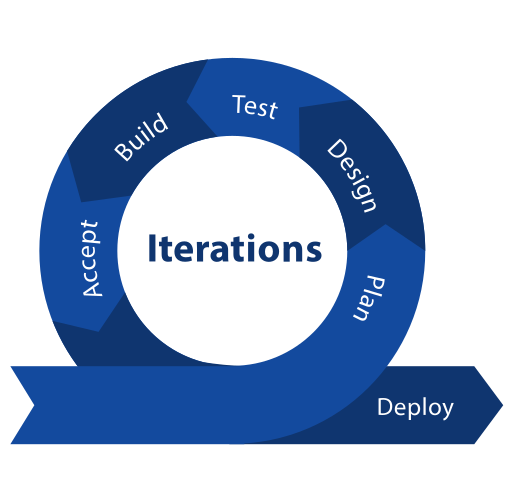
\includegraphics[width=1.1\textwidth]{img/iteration.pdf}
      \end{minipage}
      \begin{minipage}{0.49\textwidth}
        \centering
        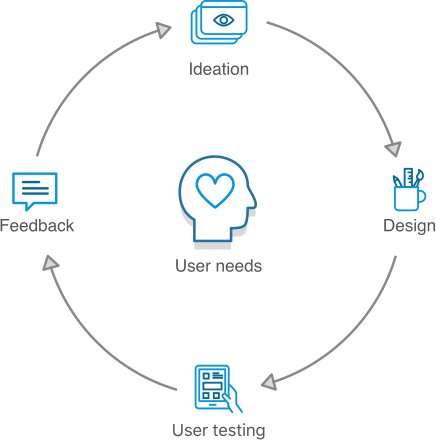
\includegraphics[width=0.9\textwidth]{img/user_centric.pdf}
      \end{minipage}
    \end{minipage}
  \end{minipage}
\end{frame}

\begin{frame}
  \frametitle{Interviews and low-fidelity prototypes -- Part I}
  \begin{minipage}{\textwidth}
    \textbf{In-person interviews and iso-standard buzzword-sallad:}
    Prototypes presented $\to$ initial ranking $\to$ iso-buzzwords sorting
    $\to$ final ranking. \\

  \end{minipage}
  \begin{minipage}{\textwidth}
    \begin{minipage}{0.49\textwidth}
      \centering
      \includegraphics[width=1.\textwidth]{../msccls/ui11.pdf}
    \end{minipage}
    \begin{minipage}{0.49\textwidth}
      \centering
      \vspace{-0.22cm}
      \hspace{-0.3cm}
      \includegraphics[width=1.\textwidth]{../msccls/ui12.pdf}
    \end{minipage}
  \end{minipage}
  The first two of four prototypes, both with a 'buttons-on-top' design.
\end{frame}

\begin{frame}
  \frametitle{Interviews and low-fidelity prototypes -- Part II}
  The remaining two prototypes with a 'buttons-on-the-side' design.
  \begin{minipage}{\textwidth}
    \begin{minipage}{0.49\textwidth}
      \centering
      \includegraphics[width=1.\textwidth]{../msccls/ui13.pdf}
    \end{minipage}
    \begin{minipage}{0.49\textwidth}
      \centering
      \vspace{-0.11cm}
      \hspace{-0.5cm}
      \includegraphics[width=1.\textwidth]{../msccls/ui14.pdf}
    \end{minipage}
  \end{minipage}
  \textbf{Goal:} Quick-and-dirty, iterate, iterate, iterate!
\end{frame}

\begin{frame}
  \frametitle{Realizing the high-fidelity prototype -- Part I}
  \begin{minipage}{\textwidth}
    \textbf{High-fidelity prototype:}
    Based on winning prototype. Created using Python, Flask and SVG-markup
    (\textbf{S}calable \textbf{V}ector \textbf{G}raphics).
  \end{minipage} \\

  \begin{minipage}{\textwidth}
    \begin{minipage}{\textwidth}
      \begin{minipage}{0.48\textwidth}
        \includegraphics[width=0.9\textwidth]{../msccls/ui14.pdf}
      \end{minipage}
      \begin{minipage}{0.02\textwidth}
        \hspace{-0.8cm}
        $\rightarrow$
      \end{minipage}
      \begin{minipage}{0.48\textwidth}
        \hspace{-0.7cm}
        \vspace{ 0.05cm}
        \includegraphics[width=0.98\textwidth]{../msccls/figures/captures/webapp_main_statistics.pdf}
      \end{minipage}
    \end{minipage}
  \end{minipage}
  Capture done by printing it through Google Chrome.
\end{frame}

\begin{frame}
  \frametitle{Realizing the high-fidelity prototype -- Part II}
  \vspace{-1cm}
  \begin{minipage}{\textwidth}
    \textbf{Hardest Task:} Employee Hours, non-outlier group (\#r$\leq$15) slightly
    above 50\% success-rate.
  \end{minipage} \\
  \begin{minipage}{\textwidth}
    \begin{minipage}{\textwidth}
      \begin{minipage}{0.49\textwidth}
        \includegraphics[width=\textwidth]{../msccls/figures/captures/webapp_employee_hours_task.pdf}
      \end{minipage}
      \begin{minipage}{0.49\textwidth}
        \includegraphics[width=\textwidth]{../msccls/figures/captures/webapp_dependencies_task.pdf}
      \end{minipage}
    \end{minipage}
  \end{minipage}
  \vspace{0.1cm}\\ \textbf{Easiest:} Task dependencies, success-rate slightly above 90\% for same group.
\end{frame}

\begin{frame}
  \frametitle{Interesting Results}
  \vspace{-1.1cm}
  Some if the basic data that was gathered during the test-period. \\
  \vspace{0.3cm}
  \begin{minipage}{\textwidth}
    \begin{minipage}{0.50\textwidth}
      \vspace{-0.2cm}
      \textit{Participants over time:} \\
      \includegraphics[width=\textwidth]{../msccls/figures/participantsOverTime.pdf}
    \end{minipage}
    \begin{minipage}{0.50\textwidth}
      \textit{Number of tests run:} \\
      \includegraphics[width=\textwidth]{../msccls/figures/testsPerUser.pdf}
    \end{minipage}
  \end{minipage} \\
  \begin{minipage}{\textwidth}
    \begin{minipage}{0.50\textwidth}
      \vspace{-0.3cm}
      \textit{Test run order:} \\
      \includegraphics[width=\textwidth]{../msccls/figures/testsRunOrder.pdf}
    \end{minipage}
    \begin{minipage}{0.50\textwidth}
      \vspace{-0.1cm}
      \textit{Completion times:} \\
      \includegraphics[width=\textwidth]{../msccls/figures/testsTimeGroupingsTotal.pdf}
    \end{minipage}
  \end{minipage} \\
\end{frame}

\begin{frame}
  \frametitle{Conclusions and realizations}
  \centering
  \begin{minipage}{.7\textwidth}
    \hspace{-0.3cm}
    \begin{minipage}{0.05\textwidth}
      
\includegraphics[width=\textwidth]{img/plan.pdf}
    \end{minipage}
    \begin{minipage}{0.05\textwidth}
      \includegraphics[width=\textwidth]{img/boxes.pdf}
    \end{minipage}
    \hspace{0.15cm}
    --
    \hspace{0.15cm}
    \begin{minipage}{0.9\textwidth}
      It was surprisingly easy to setup and gather real user-data with the
      selected technology stack.
    \end{minipage}
  \end{minipage}

  \vspace{0.8cm} \\

  \begin{minipage}{0.7\textwidth}
    \hspace{-0.3cm}
    \begin{minipage}{0.05\textwidth}
      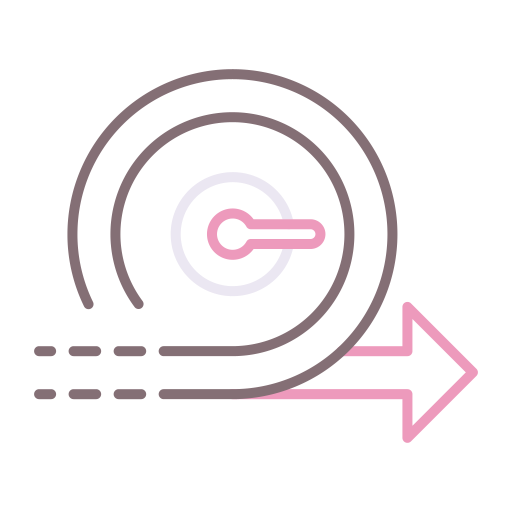
\includegraphics[width=\textwidth]{img/iterationsmall.pdf}
    \end{minipage}
    \begin{minipage}{0.05\textwidth}
      
\includegraphics[width=\textwidth]{img/train.pdf}
    \end{minipage}
    \hspace{0.15cm}
    --
    \hspace{0.15cm}
    \begin{minipage}{0.9\textwidth}
      Keeping up iterative momentum is hard, especially with low domain
      experience and a hands-off framework.
    \end{minipage}
  \end{minipage}

  \vspace{0.8cm} \\

  \begin{minipage}{.7\textwidth}
    \hspace{-0.3cm}
    \begin{minipage}{0.05\textwidth}
      \includegraphics[width=\textwidth]{img/testing.pdf}
    \end{minipage}
    \begin{minipage}{0.05\textwidth}
      
\includegraphics[width=\textwidth]{img/globe.pdf}
    \end{minipage}
    \hspace{0.15cm}
    --
    \hspace{0.15cm}
    \begin{minipage}{0.9\textwidth}
      It is possible for a single developer to lay the groundwork for a
      internet-based usability-testing platform.
    \end{minipage}
  \end{minipage}

  \vspace{0.8cm} \\

  \begin{minipage}{.7\textwidth}
    \hspace{-0.3cm}
    \begin{minipage}{0.05\textwidth}
      
\includegraphics[width=\textwidth]{img/connect.pdf}
    \end{minipage}
    \begin{minipage}{0.05\textwidth}
      \includegraphics[width=\textwidth]{img/slice.pdf}
    \end{minipage}
    \hspace{0.15cm}
    --
    \hspace{0.15cm}
    \begin{minipage}{0.9\textwidth}
      Connect it end-to-end as fast as possible in order to get a
      'vertical-slice' in front of users as soon as possible.
    \end{minipage}
  \end{minipage}
\end{frame}

\begin{frame}
  \frametitle{The End -- Questions}
  \begin{center}
    {\huge
    Thank you for listening! \\
    \vspace{1cm}
    Questions?
    }
  \end{center}
\end{frame}

\end{document}
